\documentclass[a4paper, article]{article}
\usepackage[utf8]{inputenc}
\usepackage[a4paper,total={6in, 8in}]{geometry}
\usepackage[brazil]{babel}
\usepackage{graphicx}
\usepackage{setspace}
\onehalfspacing

\begin{document} 
    \title{\vspace{-3cm}Atividade de Seminários II}
    \author{Luiz Junio Veloso Dos Santos\\ Ciência da Computação}
    \date{Setembro de 2018}
    \maketitle

    \begin{enumerate}
        {\large \item \textbf{Jantar dos Filósofos:}}\\
            \begin{figure}[h]
                \centering
                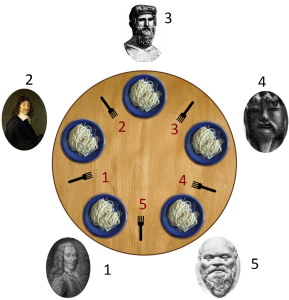
\includegraphics[width=5cm]{Imagens/jdf.png}
            \end{figure}
            \begin{enumerate}
                \item \textbf{O que é?}\\
                O jantar dos filósofos é um tipo de problema clássico na Computação, criado
                em 1965 por Edsger Dijkstra que diz:\\
                
                Imagine que existem 5 filósofos que só fazem 2 coisas na vida, comer e pensar.
                Um dia esses filósofos dividem uma mesa redonda com 5 lugares, cada lugar pertence
                a um filósofo. No centro da mesa encontra-se uma tigela de macarrão e 
                estão 5 garfos na mesa, um para cada filósofo, contudo cada filósofo só come com 2
                garfos.\\
                Quando um filósofo pensa, ele não interage com os seus colegas. Com o passar do tempo,
                cada filósofo fica com fome e tenta apanhar os dois garfos que estão mais próximos
                (Os que estão ou à esquerda ou à direita). O filósofo apenas pode apanhar um garfo
                de cada vez, e por isso não pode apanhar um garfo se este estiver na mão do vizinho.\\
                Quando um filósofo esfomeado tiver 2 garfos ao mesmo tempo, ele come sem largar os garfos.
                Apenas quando termina de comer que ele deixa os garfos novamente sobre a mesa, e em seguida
                volta a pensar novamente.\\ 

                O problema é encontrar uma forma que nenhum filósofo morra de fome.
                \newpage
                \item Uma solução:\\
                Para isso, o jantar será modelado usando uma \textit{thread} para representar cada filósofo 
                e usaremos semáforos para representar cada garfo. Quando um filósofo tenta agarrar 
                um garfo executa uma operação \textit{wait} no semáforo, quando o filósofo larga o garfo 
                executa uma operação \textit{signal} nesse mesmo semáforo. Cada filósofo (\textit{thread}) 
                vai seguir o algoritmo, ou seja, todos fazem as mesmas ações.
                O fato de seguirem o mesmo algoritmo pode dar pretexto à situação de \textit{deadlock}, dai
                a utilização das primitivas de sincronização \textit{wait} e \textit{signal}. Uma outra possibilidade 
                de \textit{deadlock} seria o fato de mais do que um filósofo ficar com fome ao mesmo tempo,
                os filósofos famintos tentariam agarrar os garfos ao mesmo tempo. Isto é outro ponto que uma
                solução satisfatória terá que ter em atenção, devendo ser salvaguardado o fato de um filósofo
                não morrer à fome. 
                Devemos recordar que uma solução livre de deadlock não elimina necessariamente
                a possibilidade de um filósofo morrer esfomeado.\\

                Obs: \textit{Deadlock} é definido como: Um conjunto de processos do Sistema Operacional está em
                situação de \textit{Deadlock} se todo processo pertencente ao conjunto estiver esperando por um
                evento que somente outro processo desse mesmo conjunto poderá fazer acontecer. 


            \end{enumerate}
        \item Problema Produtor-Consumidor:
            \begin{enumerate}
                \item\textbf{O que é?:}\\
                    O problema do Produtor-Consumidor é um clássico prolema que consiste de 2 processos
                    independentes do outro, o produtor e o consumidor, que compartilham uma mesma memória
                    (\textit{buffer}). O produtor insere dados na memória, e o consumidor retira dados na memória.
                    Os problemas são:
                    \begin{enumerate}
                        \item Tanto o produtor e o consumidor ficam acessando a memoria; 
                        \item O produtor pode tentar inserir dados na memória, mesmo estando cheia;
                        \item O consumidor pode tentar obter dados da memória, mesmo que esteja vazia;
                    \end{enumerate}
                \item\textbf{Solução:}\\
                    O produtor entrar em pausa quando a memória estiver cheia, e o consumidor entrar em pausa
                    quando a memória estiver cheia.
                \item\textbf{Tipo de situação real:}\\
                    Uma empresa de transportes que necessita de uma solução para melhorar o processo de
                    atendimento a pedidos. Nesse caso, teria uma memória com capacidade de 5000 pedidos, que
                    fica recebendo a qualquer momento por pedidos (Produtores), e um outro sistema iria coletar esses
                    pedidos para serem processados (Consumidor).
            \end{enumerate}
    \end{enumerate}

\end{document}
